\ylDisplay{Münt tassis} % Ülesande nimi
{Tundmatu autor} % Autor
{piirkonnavoor} % Voor
{2001} % Aasta
{P 1} % Ülesande nr.
{1} % Raskustase
{
% Teema: Valgusõpetus
\ifStatement
Tassi põhjas asub münt. Kui eemalduda tassist, siis teatud kaugusel kaob münt tassi serva varju. Kui aga nüüd valada tassi vett, siis võime uuesti münti samast vaatepunktist näha. Seletage antud nähtust.
\fi

\ifHint
Ülesande lahendus peitub murdumisseaduses.
\fi


\ifSolution
Vee optiline tihedus on suurem kui õhu oma. Järelikult, kui kiir väljub veest õhku, kaldub ta veepinna normaalist eemale ehk teiste sõnadega on murdumisnurk langemisnurgast suurem. Järelikult saab vaatleja samast punktist, kus ta tühja tassi puhul nägi ainult mündi punkti $A$, näha mündi punkti $C$. Vaatleja seisukohalt paistab asi nii, nagu asuks münt väiksemal sügavusel kui ta tegelikult asub. Võib näidata, et tegeliku ja näilise sügavuste suhe on $H/h$ $ = n$, kus $n$ on vee murdumisnäitajaga.
\begin{center}
	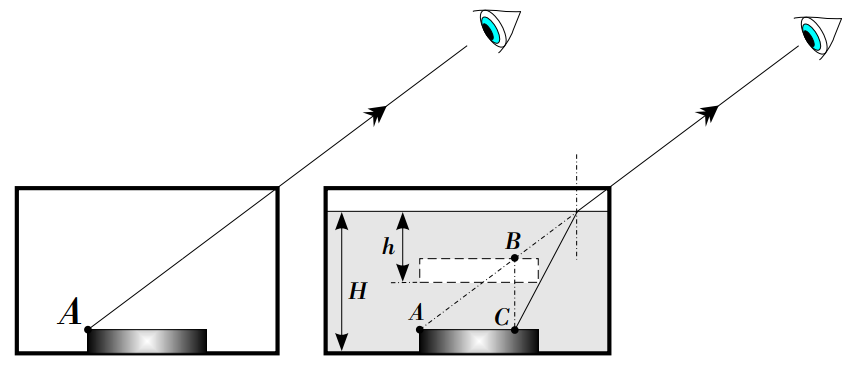
\includegraphics[width=0.5\linewidth]{2001-v2p-01-lah.PNG}
\end{center}
\fi
}